\subsection*{2.1}
%    1. Build a common-source MOS amplifier as shown below using BS170 transistor.
%Element values: R1 = R2 = 100 k, R3 = R4 = 470 , RL = 1 k, C1 = 1 µF, C2 = 100 µF,
%C3 = 10 µF. Use VDD = 15 V.
A common-source MOS amplifier as shown in figure X below using BS170 transistor, R$_1$ = R$_2$ = 100 k$\Omega$, R$_3$ = R$_4$ = 470 $\Omega$, R$_L$ = 1 k$\Omega$, C$_1$ = 1 $\mu$F, C$_2$ = 100 $\mu$F, C$_3$ = 10 $\mu$F and V$_DD$ = 15 V was built using the NI Elvis experimental setup. MUNA AÐ SETJA MÆLDU GILDIN

    \begin{figure}[h!]
        \centering
        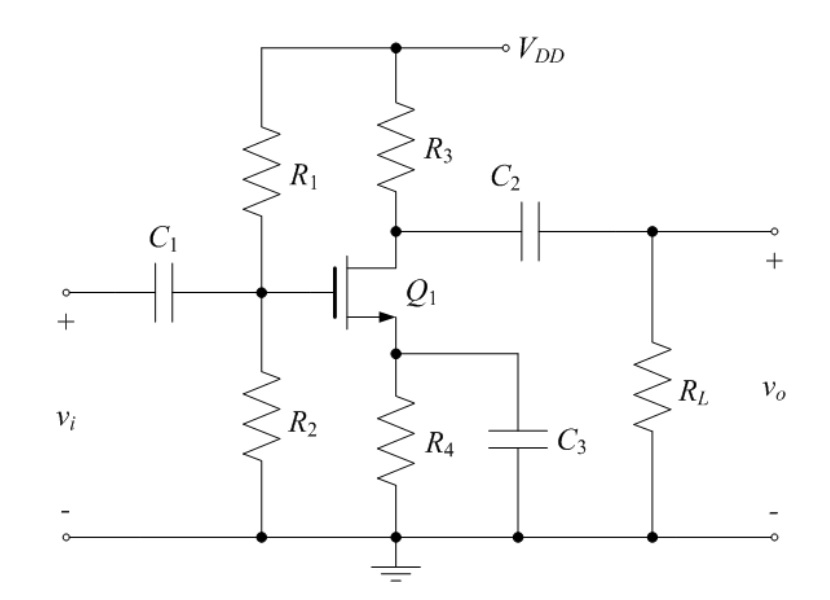
\includegraphics[width=6cm]{circuit_task_2.jpg}
        \captionof{figure}{Circuit built in task 2}
    \end{figure}



\subsection*{2.2}

%2. Use Bode Analyzer to measure the AC characteristic of the amplifier in the frequency
%range 10 Hz to 50 kHz. Use 10 steps per decade and input signal amplitude of 50 mV.
%Find the lower 3dB frequency of the circuit.

A Bode Analyzer was used to measure the AC characteristic of the amplifier in the frequency range 10 Hz to 50 kHz using 10 steps per decade and input signal amplitude of 50 mV. The result of this analysis is shown in figure X.

    \begin{figure}[h!]
        \centering
        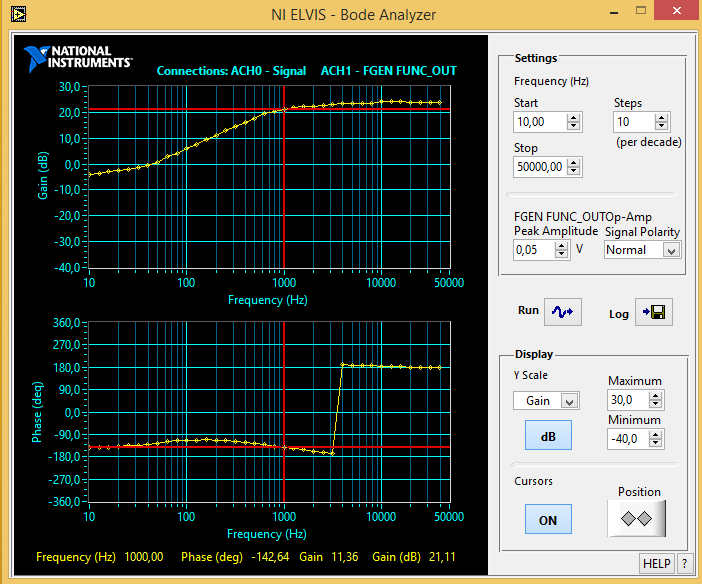
\includegraphics[width=6cm]{Task2-2-1.png}
        \captionof{figure}{AC characteristics of the amplifier showing the lower 3dB frequency of the circuit}
    \end{figure}

    \begin{figure}[h!]
        \centering
        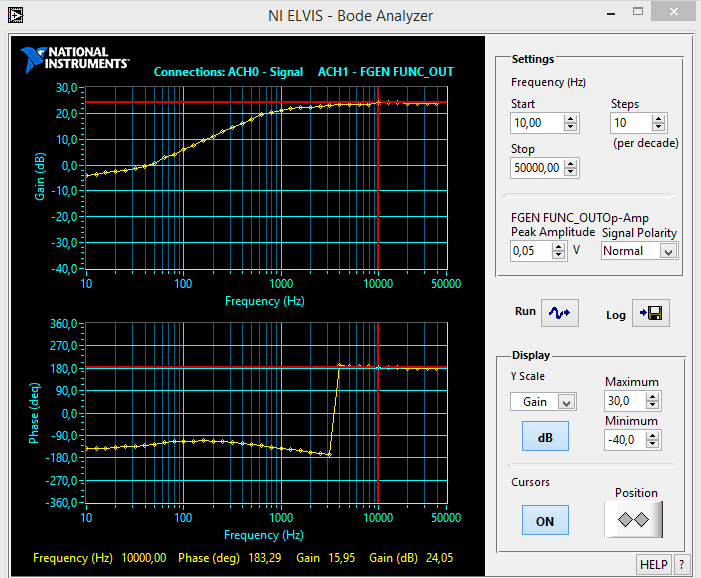
\includegraphics[width=6cm]{Task2.png}
        \captionof{figure}{AC characteristics of the amplifier showing the midband gain of the circuit}
    \end{figure}

From figure X, the 3dB frequency can be seen as 1000 kHz and the midband gain $A_1 = 24.05 dB = 10^{24.05/20) \frac{V}{V} = 15.94 \frac{V}{V}}$

\subsection*{2.3}
%3. Determine the following parameters of the circuit (at the frequency 1 kHz): voltage gain,
%input resistance, output resistance. Input signal amplitude should be small, e.g., 50 mV.
%Observe and store the input and output signal waveforms using oscilloscope.


\subsection*{2.4}
% 4. Using the transistor parameters obtained in Task 1, determine the values of gain,
%input/output resistance and the lower 3dB frequency theoretically compare them to the
%values obtained experimentally.

The transistor parameters obtained in Task 1 were used to determine the values of gain, input/output resistance and the lower 3dB frequency theoretically. Calculations can be seen in appendix I.\\

\begin{table}[htbp]
    \centering
        \begin{tabular}{ c | c | c }
        \hline
        Circuit Parameters     &   Theory                  & Simulation \\
        \hline
        Midband voltage gain    &   X $\frac{V}{V}$    &   15.95$\frac{V}{V}$\\
        Lower 3dB frequency     &   X Hz                &   1000 Hz\\
        Input Resistance        &   X k$\Omega$           &   X k$\Omega$\\
        Output Resistance       &   X k$\Omega$            &   X k$\Omega$\\
        \end{tabular}%
    \caption{Theoretical parameters compared to experimental parameters.}
    \label{tab:addlabel}%
\end{table}%

Parameters obtained by experimentally agree with those determined theoretically.?